\documentclass[10pt]{beamer}

\usetheme{Madrid}
\usecolortheme{default}

% Base packages
%\usepackage{helvet}
\usepackage{amsmath,amssymb,amsthm,mathtools,subcaption}
\usepackage{tikz,pgfplots,tabularx,booktabs}
\usepackage{unicode-math}
\usepackage{mathrsfs}
\usetikzlibrary{arrows.meta, positioning, quotes}

\usepackage{xcolor}

%\usepackage[cache=false]{minted}
%\renewcommand{\theFancyVerbLine}{\sffamily\textcolor[rgb]{0.5,0.5,1.0}{\scriptsize\oldstylenums{\arabic{FancyVerbLine}}}}
%\definecolor{bg}{rgb}{.95,.95,.95}

% Font settings
\renewcommand{\familydefault}{\sfdefault}

% TikZ libraries
\usetikzlibrary{calc,positioning,backgrounds,decorations.pathreplacing}
\pgfplotsset{compat=1.14}

% Colors
\definecolor{deepblue}{RGB}{42,39,155}
\definecolor{lightpink}{RGB}{255,240,240}
\definecolor{lightgreen}{RGB}{240,255,240}
\definecolor{lightyellow}{RGB}{255,255,240}
\definecolor{codegray}{RGB}{245,245,245}
\definecolor{codegreen}{rgb}{0,0.6,0}
\definecolor{codepurple}{rgb}{0.58,0,0.82}

% Beamer settings
\setbeamercolor{title}{fg=white,bg=deepblue}
\setbeamercolor{frametitle}{fg=white,bg=deepblue}
\setbeamercolor{section in head/foot}{fg=white,bg=deepblue}

\setbeamertemplate{footline}[text line]{%
  \parbox{\linewidth}{\vspace*{-8pt}
  %\hfill\href{https://github.com/chang-ye-tu/fin}{https://github.com/chang-ye-tu/fin}
    \hfill
   \insertframenumber~/ \inserttotalframenumber}}
\setbeamertemplate{navigation symbols}{}%[only frame symbol]

\definecolor{foo}{rgb}{.2,.2,.7}
\AtBeginSection[]{
  \begin{frame}
  \vfill
  \centering
  \begin{beamercolorbox}[sep=8pt,center,shadow=true,rounded=true]{section page}
    \usebeamerfont{title}%
    {\color{foo} \insertsectionhead}\par%
  \end{beamercolorbox}
  \vfill
  \end{frame}
}

% https://tex.stackexchange.com/questions/30423/bibliography-in-beamer
\setbeamertemplate{bibliography entry title}{}
\setbeamertemplate{bibliography entry location}{}
\setbeamertemplate{bibliography entry note}{}

\newcommand{\ds}{\displaystyle}
\newcommand{\ie}{\;\Longrightarrow\;}
\newcommand{\ifff}{\;\Longleftrightarrow\;}
\newcommand{\orr}{\;\vee\;}
\newcommand{\andd}{\;\wedge\;}
\newcommand{\mi}{\mathrm{i}}
\newcommand{\llt}{\left\langle}
\newcommand{\rgt}{\right\rangle}
\DeclareMathOperator*{\dom}{dom}
\DeclareMathOperator*{\codom}{codom}
\DeclareMathOperator*{\ran}{ran}
\DeclareMathOperator*{\sgn}{sgn}
\DeclareMathOperator*{\degr}{deg}
\DeclareMathOperator*{\jac}{D}
\newcommand{\floor}[1]{\lfloor #1 \rfloor}
\newcommand{\ceil}[1]{\lceil #1 \rceil}
%\newcommand{\proj}[2]{\mathrm{proj}_{\,#2}\,#1}

\DeclareMathOperator*\prb{\mathsf{P}}
\DeclareMathOperator*\expc{\mathsf{E}}
\DeclareMathOperator*\var{var}
\DeclareMathOperator*\cov{cov}
\DeclareMathOperator*{\argmax}{\arg\!\max}
\DeclareMathOperator*{\argmin}{\arg\!\min}
\DeclareMathOperator*{\im}{Im}
\DeclareMathOperator*{\re}{Re}
\DeclareMathOperator*{\conv}{conv}
\DeclareMathOperator*{\proj}{proj}
\DeclareMathOperator*{\tr}{tr}
\DeclareMathOperator*{\diag}{diag}
\DeclareMathOperator*{\epi}{epi}
\DeclareMathOperator*{\dist}{dist}

\theoremstyle{definition}
\newtheorem*{dfn}{Definition}
\newtheorem*{prp}{Property}
\newtheorem*{thm}{Theorem}
\newtheorem*{ex}{Example}
\newtheorem*{sol}{Solution}
\newtheorem*{prf}{Proof}
\newtheorem*{rmk}{Remark}

\usepackage{multicol}

%%%%%%%%%%%%%%%%%%%%%%%%%%%%%%%%%%%%%%%%%%%%%%%%%%%%%%%%%%%%%
% from clp3

\newcommand{\vr}{\mathbf{r}}
\newcommand{\vR}{\mathbf{R}}
\newcommand{\va}{\mathbf{a}}
\newcommand{\vb}{\mathbf{b}}
\newcommand{\vc}{\mathbf{c}}
\newcommand{\vd}{\mathbf{d}}
\newcommand{\ve}{\mathbf{e}}
\newcommand{\vC}{\mathbf{C}}
\newcommand{\vp}{\mathbf{p}}
\newcommand{\vn}{\mathbf{n}}
\newcommand{\vu}{\mathbf{u}}
\newcommand{\vv}{\mathbf{v}}
\newcommand{\vV}{\mathbf{V}}
\newcommand{\vx}{\mathbf{x}}
\newcommand{\vX}{\mathbf{X}}
\newcommand{\vy}{\mathbf{y}}
\newcommand{\vz}{\mathbf{z}}
\newcommand{\vf}{\mathbf{f}}
\newcommand{\vF}{\mathbf{F}}
\newcommand{\vg}{\mathbf{g}}
\newcommand{\vG}{\mathbf{G}}
\newcommand{\vH}{\mathbf{H}}
\newcommand{\vM}{\mathbf{M}}
\newcommand{\vT}{\mathbf{T}}
\newcommand{\vN}{\mathbf{N}}
\newcommand{\vL}{\mathbf{L}}
\newcommand{\vA}{\mathbf{A}}
\newcommand{\vB}{\mathbf{B}}
\newcommand{\vD}{\mathbf{D}}
\newcommand{\vE}{\mathbf{E}}
\newcommand{\vJ}{\mathbf{J}}
\newcommand{\vZero}{\mathbf{0}}
\newcommand{\vPhi}{\mathbf{\Phi}}
\newcommand{\vOmega}{\mathbf{\Omega}}
\newcommand{\vTheta}{\mathbf{\Theta}}
\newcommand{\cA}{\mathcal{A}}
\newcommand{\cB}{\mathcal{B}}
\newcommand{\cM}{\mathcal{M}}
\newcommand{\cO}{\mathcal{O}}
\newcommand{\cR}{\mathcal{R}}
\newcommand{\cS}{\mathcal{S}}
\newcommand{\cT}{\mathcal{T}}
\newcommand{\cU}{\mathcal{U}}
\newcommand{\cV}{\mathcal{V}}
\newcommand{\cW}{\mathcal{W}}
\newcommand{\cX}{\mathcal{X}}
%\newcommand{\hi}{\hat{\mathbf{i}}}
%\newcommand{\hj}{\hat{\mathbf{j}}}
\newcommand{\hi}{\widehat{\pmb{\imath}}}
\newcommand{\hj}{\widehat{\pmb{\jmath}}}
\newcommand{\hk}{\widehat{\mathbf{k}}}
\newcommand{\hn}{\widehat{\mathbf{n}}}
\newcommand{\hr}{\widehat{\mathbf{r}}}
\newcommand{\hvt}{\widehat{\mathbf{t}}}
\newcommand{\hN}{\widehat{\mathbf{N}}}
\newcommand{\vth}{{\pmb{\theta}}}
\newcommand{\vTh}{{\pmb{\Theta}}}
%\newcommand{\vnabla}{\pmb{\nabla}}
\newcommand{\vnabla}{   { \mathchoice{\pmb{\nabla}}
                            {\pmb{\nabla}}
                            {\pmb{\scriptstyle\nabla}}
                            {\pmb{\scriptscriptstyle\nabla}} }   }
\newcommand{\ha}[1]{\mathbf{\hat e}^{(#1)}}

\newcommand{\bbbc}{\mathbb{C}}

\newcommand{\Om}{\Omega}
\newcommand{\om}{\omega}
\newcommand{\vOm}{\pmb{\Omega}}
\newcommand{\svOm}{\pmb{\scriptsize\Omega}}
\newcommand{\al}{\alpha}
\newcommand{\be}{\beta}
\newcommand{\de}{\delta}
\newcommand{\ga}{\gamma}
\newcommand{\ka}{\kappa}
\newcommand{\la}{\lambda}

\newcommand{\cC}{\mathcal{C}}
\newcommand{\bbbone}{\mathbb{1}}

\def\tr{\mathop{\rm tr}}
\newcommand{\Atop}[2]{\genfrac{}{}{0pt}{}{#1}{#2}}

%\newcommand{\pdiff}[2]{ \frac{\partial\hfil#1\hfil}{\partial #2}}
\newcommand{\pdiff}[2]{\frac{\partial #1}{\partial #2}}
\newcommand{\pdifft}[2]{\frac{\partial^2 #1}{\partial #2^2}}
\newcommand{\dblInt}{\iint}
\newcommand{\tripInt}{\iiint}
%\newcommand{\dblInt}{\int\!\!\int}
%\newcommand{\tripInt}{\int\!\!\!\int\!\!\!\int}
%\newcommand{\dblInt}{\mathop{\int\!\!\!\int}}
%\newcommand{\tripInt}{\mathop{\int\!\!\!\int\!\!\!\int}}

\newcommand{\Set}[2]{\big\{ \ #1\ \big|\ #2\ \big\}}
\newcommand{\rhof}{{\rho_{\!{\scriptscriptstyle f}}}}
\newcommand{\rhob}{{\rho_{{\scriptscriptstyle b}}}}

\renewcommand{\neg}{ {\sim} }
\newcommand{\limp}{ {\;\Rightarrow\;} }
\newcommand{\nimp}{ {\;\not\Rightarrow\;} }
\newcommand{\liff}{ {\;\Leftrightarrow\;} }
\newcommand{\niff}{ {\;\not\Leftrightarrow\;} }

\newcommand{\st}{ {\mbox{ s.t. }} }
\newcommand{\es}{ {\varnothing}}
\newcommand{\pow}[1]{ \mathcal{P}\left(#1\right) }
\newcommand{\set}[1]{ \left\{#1\right\} }

\newcommand{\bbbn}{\mathbb{N}}
\newcommand{\bbbr}{\mathbb{R}}
\newcommand{\bbbp}{\mathbb{P}}
\newcommand{\De}{\Delta}
\newcommand{\cD}{\mathcal{D}}
\newcommand{\cP}{\mathcal{P}}
\newcommand{\cI}{\mathcal{I}}
\newcommand{\veps}{\varepsilon}
\newcommand{\dee}[1]{\mathrm{d}#1}

\newcommand{\bdiff}[2]{ \frac{\mathrm{d}}{\mathrm{d}#2} \left( #1 \right)}
\newcommand{\ddiff}[3]{ \frac{\mathrm{d}^#1#2}{\mathrm{d}{#3}^#1}}
\newcommand{\half}{\tfrac{1}{2}}
\newcommand{\diff}[2]{\frac{\mathrm{d} #1}{\mathrm{d} #2}}
\newcommand{\difftwo}[2]{\frac{\mathrm{d^2} #1}{\mathrm{d}{#2}^2}}

%%%%%%%%%%%%%%%%%%%%%%%%%%%%%%%%%%%%%%%%%%%%%%%%%%%%%%%%%%%%%%%%%%%%%

\newcommand\scalemath[2]{\scalebox{#1}{\mbox{\ensuremath{\displaystyle #2}}}}

\title{Review of Prerequisite Mathematics}
\author{}
\date{}

\begin{document}

\begin{frame}
\titlepage
\end{frame}

\begin{frame}
\begin{dfn}[The Jacobian]
  Let $V$ be open in $\mathbb{R}^n$, $\vx\in V$, and $g_i:V\to\mathbb{R}$, $i = 1,\,2,\,\ldots,\,m$ be $C^1$ on $V$. The Jacobian of $\vg(\vx): \mathbb{R}^n\to\mathbb{R}^m$ is defined as
  \begin{align*}
    \jac\vg(\vx) = %\frac{\partial(g_1,\,g_2,\,\ldots,\,g_m)}{\partial (x_1,\,x_2,\,\ldots,\,x_{\!n})}(\vx) = 
    \begin{pmatrix}
      \frac{\partial g_1}{\partial x_1} & \frac{\partial g_1}{\partial x_2} & \cdots & \frac{\partial g_1}{\partial x_{\!n}} \\
      \frac{\partial g_2}{\partial x_1} & \frac{\partial g_2}{\partial x_2} & \cdots & \frac{\partial g_2}{\partial x_{\!n}} \\
      \vdots & \vdots & \ddots &\vdots \\
      \frac{\partial g_m}{\partial x_1} & \frac{\partial g_m}{\partial x_2} & \cdots & \frac{\partial g_m}{\partial x_{\!n}}
    \end{pmatrix}(\vx)
  \end{align*}
\end{dfn}
\begin{thm}%[\citet{rudin} 9.15; \citet{apostol_adv} Theorem 12.7; \citet{wade} 11.28]
  Suppose that $\vf$ and $\vg$ are vector functions. If $\vg$ is differentiable at $\va$ and $\vf$ is differentiable at $\vg(\va)$, then $\vf\circ\vg$ is differentiable at $\va$ and
  \begin{align*}
    \jac(\vf\circ\vg)(\va) = \jac\vf(\vg(\va))\,\jac\vg(\va)
  \end{align*}
  More explicitly, if $f$ is a differentiable function of $x_1,\,x_2,\,\ldots,\,x_n$, and each $x_j$ is a differentiable function of $t_1,\,t_2,\,\ldots,\,t_m$, $n$, $m\geqslant 1$; then $f$ is a differentiable function of $t_1,\,t_2,\,\ldots,\,t_m$ with
  \begin{align*}
    \pdiff{f}{t_i} = \pdiff{f}{x_1}\,\pdiff{x_1}{t_i} + \pdiff{f}{x_2}\,\pdiff{x_2}{t_i} + \cdots + \pdiff{f}{x_n}\,\pdiff{x_n}{t_i}
  \end{align*}
\end{thm}
\end{frame}

\begin{frame}
\begin{ex}
  Let $w = f(x z, y z)$, where $f$ is a differentiable function. Prove that $\ds x\frac{\partial w}{\partial x} + y\frac{\partial w}{\partial y} = z\frac{\partial w}{\partial z}$.
\end{ex}

\begin{sol}
  Write $u(x,y,z)=xz$ and $v(x,y,z)=yz$ so that $w(x,y,z) = f\big(u(x,y,z), v(x,y,z)\big)$. By the chain rule,
  \begin{align*}
    &\pdiff{w}{x}(x,y,z) = \pdiff{}{x}\big[f \big(u(x,y,z), v(x,y,z)\big)\big] \\
    &= \pdiff{f}{u}\big(u(x,y,z), v(x,y,z)\big)\pdiff{u}{x}(x,y,z) + \pdiff{f}{v}\big(u(x,y,z), v(x,y,z)\big)\pdiff{v}{x}(x,y,z) \\ 
    &= z\pdiff{f}{u}(xz, yz)
  \end{align*}
  \begin{align*}
    &\pdiff{w}{y}(x,y,z) = \pdiff{}{y}\big[f \big(u(x,y,z), v(x,y,z)\big)\big] \\
    &= \pdiff{f}{u}\big(u(x,y,z), v(x,y,z)\big)\pdiff{u}{y}(x,y,z) + \pdiff{f}{v}\big(u(x,y,z), v(x,y,z)\big)\pdiff{v}{y}(x,y,z) \\
    &= z\pdiff{f}{v}(xz, yz)
  \end{align*}
  \begin{align*}
    &\pdiff{w}{z}(x,y,z) = \pdiff{}{z}\big[f \big(u(x,y,z), v(x,y,z)\big)\big] \\
    &= \pdiff{f}{u}\big(u(x,y,z), v(x,y,z)\big)\pdiff{u}{z}(x,y,z) + \pdiff{f}{v}\big(u(x,y,z), v(x,y,z)\big)\pdiff{v}{z}(x,y,z) \\
    &= x\pdiff{f}{u}(xz, yz) + y\pdiff{f}{v}(xz, yz)
  \end{align*}
  So
  \begin{align*}
    \pdiff{w}{x} + y\pdiff{w}{y} &= xz\pdiff{f}{u}(xz, yz) + yz\pdiff{f}{v}(xz, yz) \\&= z\left[x\pdiff{f}{u}(xz, yz) + y\pdiff{f}{v}(xz, yz)\right] = z\pdiff{w}{z}
  \end{align*}
\end{sol}
\end{frame}

\begin{frame}{Unconstrained Optimization Problems}

\begin{thm}%[\citet{rudin} 4.16; \citet{apostol_adv} Theorem 4.27; \citet{wade} 9.57]
  Given $\ds S\subseteq\mathbb{R}^n$ and continuous $f: S\to\mathbb{R}$; if $S$ is compact, then  
  \begin{align*}
    M = \sup\left\{f(\vx): \vx\in S\right\}\quad\text{ and }\quad m = \inf\left\{f(\vx): \vx\in S\right\}
  \end{align*}
  are finite real numbers. Moreover, there exists points $\vx_\text{M}$, $\vx_\text{m}\in S$ such that $M = f(\vx_\text{M})$ and $m = f(\vx_\text{m})$.
\end{thm}

\begin{dfn}
  Given $\ds S\subseteq\mathbb{R}^n$, $\ds f:S\to\mathbb{R}$ and $\ds B(\vx, h)\equiv\{\vy\in\mathbb{R}^n\;|\;|\vy - \vx| < h\}$, $f$ achieves 
  \begin{itemize}
    \item global maximum $\ds f(\vx_\text{M})$ at $\ds\vx_\text{M}\in S$: $\ds f(\vx_\text{M})\geqslant f(\vx),\;\forall\,\vx\in S$. 
    \item global minimum $\ds f(\vx_\text{m})$ at $\ds \vx_\text{m}\in S$: $\ds f(\vx_\text{m})\leqslant f(\vx),\;\forall\,\vx\in S$. 
    \item local maximum $\ds f(\vx_0)$ at $\ds\vx_0\in S$: $\ds\exists\,h_0 > 0$ s.t. $\ds f(\vx_0)\geqslant f(\vx),\;\forall\,\vx\in B(\vx_0, h_0)\,\cap\,S$. 
    \item local minimum $\ds f(\vx_1)$ at $\ds\vx_1\in S$: $\ds\exists\,h_1 > 0$ s.t. $\ds f(\vx_1)\leqslant f(\vx),\;\forall\,\vx\in B(\vx_1, h_1)\,\cap\,S$. 
  \end{itemize}
\end{dfn}
\end{frame}

\begin{frame}
\begin{thm}[necessary conditions for extremum]
  Given $\ds S\subseteq\mathbb{R}^n$ and differentiable $\ds f:S\to\mathbb{R}$, if $f$ achieves extremum at an interior $\vc\in S$, then $\ds\nabla f(\vc) = \vZero$. 
\end{thm}

\begin{prf}
  If $\ds\vc = (c_1,\,c_2,\,\ldots,\,c_n)$, let 
  \begin{align*}
    g_j(t)\equiv f(c_1,\,c_2,\,\ldots,\,c_{j - 1},\,t,\,c_{j + 1},\,\ldots,\,c_n), \quad j = 1,\,2,\,\ldots,\,n 
  \end{align*}
  For $f$ achieves extremum at $\vc$, $f(\vc) = g_j(c_j)$, $g_j$ achieves extremum at $c_j\ie g_j'(t)\,\big|_{t = c_j} = 0 \ie D_j f(\vc) = 0\;\forall\,j$, so $\ds\nabla f(\vc) = \vZero$.  
\end{prf}

\begin{thm}
  Given $\ds S\subseteq\mathbb{R}^n$, if $f:S\to\mathbb{R}$ achieves extremum at $\vc\in S$, then $\vc$ can possibly be a
    \begin{itemize}
      \item critical point: $\ds \nabla f(\vc) = \vZero$. 
      \item singular point: $f$ is non-differentiable at $\vc$.  
      \item boundary point of $S$. 
    \end{itemize}
\end{thm}
\end{frame}

\begin{frame}
\begin{dfn}[Hessian Matrix]
  Given $\ds S\subseteq\mathbb{R}^n$, an interior point $\vc$ of $S$, and a differentiable function $\ds f:S\to\mathbb{R}$, 
  \begin{align*}
    \vH(f, \vc) = \begin{pmatrix}f_{11} & f_{12} & \cdots & f_{1n} \\ f_{21} & f_{22} & \cdots & f_{2n} \\ \vdots & \vdots & \ddots & \vdots \\ f_{n1} & f_{n2} & \cdots & f_{nn}\end{pmatrix}, \quad f_{ij} = \frac{\partial^2 f}{\partial x_j\partial x_i}(\vc), \quad i,\,j = 1,\,2,\,\ldots,\,n.
  \end{align*}
\end{dfn}

\begin{dfn}[Matrix Positive/Negative Definiteness] 
  Given an $n\times n$ real symmetric matrix $\vA$. For any $\ds\vv\in\mathbb{R}^n\ne\vZero$, $\vA$ is
  \begin{multicols}{2}
    \begin{itemize}
      \item positive-definite: $\ds\vv\vA\vv^\top > 0$ 
      \item negative-definite: $\ds\vv\vA\vv^\top < 0$
      \item positive-semidefinite: $\ds\vv\vA\vv^\top\geqslant 0$
      \item negative-semidefinite: $\ds\vv\vA\vv^\top\leqslant 0$
    \end{itemize}
  \end{multicols}
\end{dfn}
\end{frame}

\begin{frame}
\begin{dfn}[Minor] 
  Given an $n\times n$ matrix $\vA = \begin{pmatrix}a_{11} & a_{12} & \cdots & a_{1n} \\ a_{21} & a_{22} & \cdots & a_{2n} \\ \vdots & \vdots & \ddots & \vdots \\ a_{n1} & a_{n2} & \cdots & a_{nn} \end{pmatrix}$ and minor $\vA\begin{pmatrix}i_1,\,i_2,\,\cdots,\,i_k\\j_1,\,j_2,\,\cdots,\,j_k\end{pmatrix} = \begin{vmatrix}a_{i_1 j_1} & a_{i_1 j_2} & \cdots & a_{i_1 j_k} \\ a_{i_2 j_1} & a_{i_2 j_2} & \cdots & a_{i_2 j_k} \\ \vdots & \vdots & \ddots & \vdots \\ a_{i_k j_1} & a_{i_k j_2} & \cdots & a_{i_k j_k} \end{vmatrix}$, $1\leqslant k\leqslant n$, $1\leqslant i_1 < i_2 < \cdots < i_k \leqslant n$, $1\leqslant j_1 < j_2 < \cdots < j_k \leqslant n$. 
  \begin{itemize}
    \item $\ds\Delta_k\equiv\vA\begin{pmatrix}i_1,\,i_2,\,\cdots,\,i_k\\i_1,\,i_2,\,\cdots,\,i_k\end{pmatrix}$ is the $k$-th order principal minor of $A$. 
    \item $\ds M_k\equiv\vA\begin{pmatrix}1,\,2,\,\cdots,\,k\\1,\,2,\,\cdots,\,k\end{pmatrix}$ is the $k$-th order leading principal minor of $A$. 
  \end{itemize}
\end{dfn}

\begin{thm}[Criteria for Matrix Positive/Negative Definiteness] 
  Given an $n\times n$ real symmetric matrix $\vA$, then $\forall\,k\leqslant n$, $\vA$ is
  \vspace{-3mm}
  \begin{multicols}{2}
    \begin{itemize}
      \item positive-definite $\ifff M_k > 0$
      \item negative-definite $\ifff (-1)^k M_k> 0$
      \item positive-semidefinite $\ifff \Delta_k \geqslant 0$
      \item negative-semidefinite $\ifff (-1)^k \Delta_k \geqslant 0$
    \end{itemize}
  \end{multicols}
\end{thm}
\end{frame}

%\begin{frame}
%\begin{ex}
%  Consider the matrix $\ds\vA = \begin{pmatrix}2 & -1 & 0\\-1 & 2 & -1\\ 0 & -1 & 2\end{pmatrix}$: Let $\ds\vv = \llt a,\,b,\,c\rgt$, $\ds\vv\vA\vv^\top = \begin{pmatrix}a & b & c\end{pmatrix}\begin{pmatrix}2 & -1 & 0\\-1 & 2 & -1\\ 0 & -1 & 2\end{pmatrix}\begin{pmatrix}a\\b\\c\end{pmatrix} = \begin{pmatrix}2a - b&-a + 2b - c&-b + 2c\end{pmatrix}\cdot\\ \begin{pmatrix}a\\b\\c\end{pmatrix} = (2a - b)a + (-a + 2b - c)b + (-b + 2c)c = 2a^2-2ab+2b^2 - 2bc + 2c^2 = a^2 + (a - b)^2 + (b - c)^2 + c^2 > 0$, except when $a = b = c = 0$, so it is positive-definite. Also, $\vA$'s $M_1$, $M_2$, $M_3$ are $\ds 2,\;\begin{vmatrix}2 & -1 \\ -1 & 2\end{vmatrix} = 3,\;\begin{vmatrix}2 & -1 & 0\\-1 & 2 & -1\\ 0 & -1 & 2\end{vmatrix} = 4$ respectively, by the above criteria $\vA$ is positive-definite. 
%\end{ex}
%\end{frame}

\begin{frame}{Equalities Constrained Optimization: The Lagrange Multipliers Method}

%\begin{thm}[\citet{apostol_adv} Theorem 13.12; \citet{wade} 11.63]
%  Let $m < n$, $V$ be open in $\mathbb{R}^n$, and $f$, $g_i:V\to\mathbb{R}$, $i = 1,\,2,\,\ldots,\,m$ be $C^1$ on $V$. Suppose that $\exists\,a\in V$ s.t. the Jacobian at $a$
%  \begin{align*}
%    \frac{\partial(g_1,\,g_2,\,\ldots,\,g_m)}{\partial (x_1,\,x_2,\,\ldots,\,x_{\!m})}(a) = 
%    \begin{vmatrix}
%      \frac{\partial g_1}{\partial x_1} & \frac{\partial g_1}{\partial x_2} & \cdots & \frac{\partial g_1}{\partial x_{\!m}} \\
%      \frac{\partial g_2}{\partial x_1} & \frac{\partial g_2}{\partial x_2} & \cdots & \frac{\partial g_2}{\partial x_{\!m}} \\
%      \vdots & \vdots & \ddots &\vdots \\
%      \frac{\partial g_m}{\partial x_1} & \frac{\partial g_m}{\partial x_2} & \cdots & \frac{\partial g_m}{\partial x_{\!m}}
%    \end{vmatrix}(a) \ne 0
%  \end{align*}
%  If $f(a)$ is a local extremum of $f$ subject to the constraints $g_i(a) = 0$, $i = 1, 2, \ldots, m$, then there exist scalars $\lambda_1,\,\lambda_2,\,\ldots,\,\lambda_m$ s.t.
%  \begin{align*}
%    \nabla f(a) + \sum_{i = 1}^m \lambda_i\nabla g_i(a) = 0
%  \end{align*}
%\end{thm}

\begin{thm}%[\citet{apostol_adv} Theorem 13.12; \citet{wade} 11.63]
  Given an open set $S\subseteq\mathbb{R}^n$, differentiable functions $f:S\to\mathbb{R}$ and $g_j:S\to\mathbb{R}$, $j=1,\,2,\,\ldots,\,m$, $m < n$, and $\ds X_0 = \big\{\vx\in S\;|\;g_j(\vx) = 0,\,j=1,\,2,\,\ldots,\,m\big\}$. If $f$ has an extremum at $\ds\vx_0\in S\,\cap\,X_0$ and $\det\big(D_i g_j(\vx_0)\big)\ne 0$, then
  \begin{align*}
    \exists\,\lambda_1,\,\lambda_2,\,\ldots,\,\lambda_m\quad\text{s.t.}\quad D_i f(\vx_0) + \sum_{j = 1}^m\lambda_j D_i g_j(\vx_0) = 0,\quad\ds i = 1,\,2,\,\ldots,\,n
  \end{align*}
\end{thm}
\begin{rmk}
  Let $\ds\mathcal{L}\equiv f + \sum_{j = 1}^m \lambda_j\,g_j$, the sufficient condition can be rewritten as
  \begin{align*}
    D_i\,\mathcal{L}(\vx_0) &= 0,\quad i = 1,\,2,\,\ldots,\,n \\
    g_j(\vx_0) &= 0,\quad j=1,\,2,\,\ldots,\,m
  \end{align*}
\end{rmk}
\end{frame}

\begin{frame}
\begin{ex} 
  Find the maximum and minimum values of $\ds x^2 - 10 x - y^2$ on $\ds x^2 + 4 y^2 = 16$. 
\end{ex}

\begin{sol}
  Let $\ds\mathcal{L} = x^2 - 10 x - y^2 + \lambda\,(x^2 + 4 y^2 - 16)$, then 
  \begin{align}
    \pdiff{\mathcal{L}}{x} &= 2 x - 10 + 2\lambda x = 0\ie x - 5 + \lambda x = 0 \label{eq:1}\\
    \pdiff{\mathcal{L}}{y} &= -2y + 8\lambda y = 0\ie -y + 4\lambda y = 0 \label{eq:2} \\
    x^2 &+ 4 y^2 - 16 = 0 \label{eq:3}
  \end{align}
  From \eqref{eq:2} $(1 - 4\lambda) y = 0$, so $y = 0\orr\lambda = \frac{1}{4}$. If $y = 0$, from \eqref{eq:3} $x = \pm 4$; if $\lambda=\frac{1}{4}$, from \eqref{eq:1} $(1 + \lambda)\,x = 5\ie x = 4$, substituting into \eqref{eq:3} gives $y = 0$. Therefore, the extremum points are $(x, y) = (4, 0),\,(-4, 0)$; $x^2 - 10x - y^2$ has a maximum value of $56$ (at $(x, y) = (-4, 0)$), and a minimum value of $-24$ (at $(x, y) = (4, 0)$). 
\end{sol}
\end{frame}

%\begin{frame}
%\begin{ex}
%  Find the point on $x^2 = y^2 + z^2$ that is closest to $(0, 1, 3)$. 
%\end{ex}
%
%\begin{sol}
%  The square of the distance is $x^2 + (y - 1)^2 + (z - 3)^2$, with the constraint $x^2 - y^2 - z^2 = 0$. Let $\ds\mathcal{L} = x^2 + (y - 1)^2 + (z - 3)^2 + \lambda(x^2 - y^2 - z^2)$, then
%  \begin{align}
%    \pdiff{\mathcal{L}}{x} &= 2 x + 2\lambda x = 0\ie (1 + \lambda) x = 0 \label{eq:4}\\
%    \pdiff{\mathcal{L}}{y} &= 2\,(y - 1) - 2\lambda y = 0\ie (1 - \lambda) y = 1 \label{eq:5} \\
%    \pdiff{\mathcal{L}}{z} &= 2\,(z - 3) - 2\lambda z = 0\ie (1 - \lambda) z = 3 \label{eq:6} \\
%    x^2 &- y^2 - z^2 = 0 \label{eq:7}
%  \end{align}
%  From \eqref{eq:4} $(1 + \lambda) x = 0$, so $x = 0\orr\lambda = -1$. If $x = 0$, from \eqref{eq:7} $y = z = 0$; if $\lambda = -1$, from \eqref{eq:5} $y = \frac{1}{2}$, from \eqref{eq:6} $z = \frac{3}{2}$, substituting into \eqref{eq:7} gives $x = \pm\sqrt{\frac{5}{2}}$. Therefore, the extremum points are $(x, y, z) = (0, 0, 0),\,\Big(\pm\sqrt{\frac{5}{2}}, \frac{1}{2}, \frac{3}{2}\Big)$; the minimum value of the square of the distance $x^2 + (y - 1)^2 + (z - 3)^2$ is $5$, occurring at $(x, y, z) = \Big(\pm\sqrt{\frac{5}{2}}, \frac{1}{2}, \frac{3}{2}\Big)$. 
%\end{sol}
%\end{frame}

\begin{frame}
\begin{ex}
  Find the maximum and minimum values of $\ds f(x, y, z) = (x + z)\,e^y$ on $x^2 + y^2 + z^2 = 6$. 
\end{ex}
  
\begin{sol}
  Let $\ds\mathcal{L} = (x + z)\,e^y + \lambda\,(x^2 + y^2 + z^2 - 6)$, then \vspace{-3mm}
  \begin{align}
    \pdiff{\mathcal{L}}{x} &= e^y + 2\lambda x = 0\label{eq:13}\\
    \pdiff{\mathcal{L}}{y} &= (x + z)\,e^y + 2\lambda y = 0\label{eq:14} \\
    \pdiff{\mathcal{L}}{z} &= e^y + 2\lambda z = 0\label{eq:15} \\
    x^2 &+ y^2 + z^2 - 6 = 0 \label{eq:16}
  \end{align}

  \vspace{-3mm}
  From \eqref{eq:13}, \eqref{eq:15} $2\,\lambda(x - z) = 0$, so $\lambda = 0\orr x = z$. If $\lambda = 0$, then from \eqref{eq:13} $\ds e^y = 0$ which is impossible, so $x = z$. From \eqref{eq:13} $e^y = -2\lambda x$, substituting into \eqref{eq:14} $2x\,(-2\lambda x) + 2\lambda y = 0\ie y = 2x^2$, substituting into \eqref{eq:16} gives $x^2 + 4x^4 + x^2 = 6\ie (4x^2 + 6)(x^2 - 1) = 0 \ie x = \pm 1$. Therefore, the extremum points are $(x, y, z) = (1, 2, 1),\;(-1, 2, -1)$; $(x + z)\,e^y$ has a maximum value of $2e^2$ (at $(x, y, z) = (1, 2, 1)$), and a minimum value of $-2e^2$ (at $(x, y, z) = (-1, 2, -1)$). 
\end{sol}
\end{frame}

\begin{frame}
\begin{ex}
  If $L$ is the curve of intersection of $\scalemath{0.95}{z^2 = x^2 + y^2}$ and $\scalemath{0.95}{x - 2z = 3}$, find the point on $L$ that is closest to the origin and the shortest distance. 
\end{ex}

\begin{sol}
  The objective is $\scalemath{0.95}{x^2 + y^2 + z^2}$ with constraints $\scalemath{0.95}{x^2 + y^2 - z^2 = 0}$ and $\scalemath{0.95}{x - 2z - 3 = 0}$. Let $\ds\scalemath{0.95}{\mathcal{L} = x^2 + y^2 + z^2 + \lambda_1\,(x^2 + y^2 - z^2) + \lambda_2\,(x - 2z - 3)}$, then \vspace{-3mm}
  \begin{align}
    \scalemath{0.95}{\pdiff{\mathcal{L}}{x}} &\scalemath{0.95}{= 2 x + 2\lambda_1 x + \lambda_2 = 0 \ie 2\,(1 + \lambda_1) x + \lambda_2 = 0}\label{eq:8}\\
    \scalemath{0.95}{\pdiff{\mathcal{L}}{y}} &\scalemath{0.95}{= 2 y + 2\lambda_1 y = 0 \ie (1 + \lambda_1)y = 0}\label{eq:9} \\
    \scalemath{0.95}{\pdiff{\mathcal{L}}{z}} &\scalemath{0.95}{= 2 z - 2\lambda_1 z - 2\lambda_2 = 0 \ie (1 - \lambda_1)z - \lambda_2 = 0}\label{eq:10}\\
    \scalemath{0.95}{x^2} &\scalemath{0.95}{+ y^2 - z^2 = 0}\label{eq:11} \\
    \scalemath{0.95}{x} &\scalemath{0.95}{- 2z - 3 = 0}\label{eq:12}
  \end{align}
  
  \vspace{-3mm}
  From \eqref{eq:9} $(1 + \lambda_1) y = 0$, so $y = 0\orr\lambda_1 = -1$. If $y = 0$, from \eqref{eq:11} $x^2 = z^2 \ie x = \pm z$. If $x = z$, from \eqref{eq:12} $x = z = -3$. If $x = -z$, from \eqref{eq:12} $x = 1$, $z = -1$; if $\lambda_1 = -1$, from \eqref{eq:8} $\lambda_2 = 0$, from \eqref{eq:10} $z = 0$, substituting into \eqref{eq:11} gives $x = y = 0$, which contradicts \eqref{eq:12}. Therefore, the extremum points are $(x, y, z) = (-3, 0, -3),\,(1, 0, -1)$; optimizer: $(1, 0, -1)$.
\end{sol}
\end{frame}

\begin{frame}{Affine Set}
\begin{itemize}
  \item {\bf line} through $x_1$, $x_2$: all points of the form $\ds x = \theta x_1 + (1 - \theta) x_2$, $\theta\in\mathbb{R}$
  \item {\bf affine set} contains the line through any two distinct points in the set
  \item e.g. solution set of linear equations $\ds\{x\,|\,Ax = b\}$; every affine set can be expressed as solution set of system of linear equations
\end{itemize}

\begin{figure}[!htbp]
  \centering
  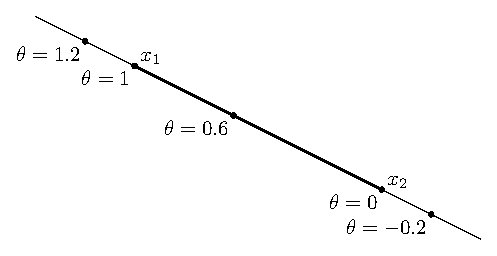
\includegraphics[scale=0.75,page=1]{fig/note06/02.pdf}
  %\caption{$y = \sin x$,$y = \sin^{-1} x$}
\end{figure}

\end{frame}

\begin{frame}{Convex Set}
\begin{itemize}
  \item {\bf line segment} through $x_1$, $x_2$: all points of the form \\$\ds x = \theta x_1 + (1 - \theta) x_2$, $0\leqslant\theta\leqslant 1$
  \item {\bf convex set} contains the line segment between any two distinct points in the set: \\$\ds x_1,\,x_2\in S\ie \forall\,0\leqslant\theta\leqslant 1,\;\theta x_1 + (1 - \theta) x_2\in S$
\end{itemize}

\begin{figure}[!htbp]
  \centering
  \includegraphics[scale=1,page=2]{fig/note06/02.pdf}
  %\caption{$y = \sin x$,$y = \sin^{-1} x$}
\end{figure}

\end{frame}

\begin{frame}{Convex Combination, Convex Hull}

\begin{itemize}
  \item {\bf convex combination} of $x_1$, $x_2$, $\ldots$, $x_k$: any point $x$ of the form $x = \theta_1 x_1 + \theta_2 x_2 + \cdots + \theta_k x_k$ with $\theta_1 + \theta_2 + \cdots + \theta_k = 1$, $\theta_i\geqslant 0$
  \item {\bf convex hull} $\conv S$: sets of all convex combinations of points in $S$
\end{itemize}

\begin{figure}[!htbp]
  \centering
  \includegraphics[scale=1,page=3]{fig/note06/02.pdf}
  %\caption{$y = \sin x$,$y = \sin^{-1} x$}
\end{figure}

\end{frame}

\begin{frame}{Convex Cone}
\begin{itemize}
  \item {\bf conic (nonnegative) combination} of $x_1$ and $x_2$: any point $x$ of the form $x = \theta_1 x_1 + \theta_2 x_2$ with $\theta_i\geqslant 0$
  \item {\bf convex cone} set that contains all conic combinations of points in the set
\end{itemize}

\begin{figure}[!htbp]
  \centering
  \includegraphics[scale=0.9,page=4]{fig/note06/02.pdf}
  %\caption{$y = \sin x$,$y = \sin^{-1} x$}
\end{figure}

\end{frame}

\begin{frame}{Hyperplane, Halfspace}
\begin{itemize}
  \item {\bf hyperplane}: set of the form $\ds\{x\,|\,a^\top x = b\}$ with $a\ne 0$
  \item {\bf halfspace}: set of the form $\ds\{x\,|\,a^\top x\leqslant b\}$ with $a\ne 0$
  \item $a$: normal vector \\ hyperplanes are affine and convex, halfspaces are convex 
\end{itemize}

\begin{figure}[!htbp]
  \centering
  \includegraphics[scale=0.9,page=6]{fig/note06/02.pdf}
  \includegraphics[scale=0.7,page=7]{fig/note06/02.pdf}
  %\caption{$y = \sin x$,$y = \sin^{-1} x$}
\end{figure}

\end{frame}

\begin{frame}{Euclidean Ball, Ellipsoid}
\begin{itemize}
  \item {\bf (Euclidean) ball} with center $x_c$ and radius $r$: \\ $\ds B(x_c, r) = \{x\,|\,\|x - x_c\|_2\leqslant r\} = \{x_c + r\,u\,|\,\|u\|_2 \leqslant 1\}$
  \item {\bf ellipsoid}: set of the form $\ds\{x\,|\,(x - x_c)^\top P^{-1}(x - x_c)\leqslant 1\}$ with $P\in\mathsf{S}_{++}^n$ ($P$ symmetric positive definite), or $\ds\{x_c + A\,u\,|\,\|u\|_2 \leqslant 1\}$ with nonsingular $A$
\end{itemize}

\begin{figure}[!htbp]
  \centering
  \includegraphics[scale=0.9,page=9]{fig/note06/02.pdf}
  \caption{$y = \sin x$, $y = \sin^{-1} x$}
\end{figure}

\end{frame}

\begin{frame}{Norm Ball, Norm Cone}
\begin{itemize}
  \item {\bf norm}: a function $\|\cdot\|$ that satisfies 
    \begin{itemize}
      \item $\|x\|\geqslant 0$; $\|x\| = 0\ifff x = 0$
      \item $\|tx\| = |t|\|x\|$, $\forall\,t\in\mathbb{R}$
      \item $\|x + y\|\leqslant\|x\| + \|y\|$
    \end{itemize}
  \item {\bf norm ball} with center $x_c$ and radius $r$: $\ds\{x\,|\,\|x - x_c\|\leqslant r\}$
  \item {\bf norm cone}: $\ds\{(x, t)\,|\,\|x\|\leqslant t\}$
  \item norm balls and norm cones are convex
  \item notation for different norms: $\|\cdot\|_2$, $\|\cdot\|_{\text{symb}}$
\end{itemize}

\begin{figure}[!htbp]
  \centering
  \includegraphics[scale=0.9,page=9]{fig/note06/02.pdf}
  %\caption{$y = \sin x$,$y = \sin^{-1} x$}
\end{figure}

\end{frame}

\begin{frame}{Polyhedra}
\begin{itemize}
  \item {\bf polyhedron}: solution set of finitely many linear equalities and inequalities $\ds\{x\,|\,A\,x\preccurlyeq b,\, C\,x = d\}$, where $\ds A\in\mathbb{R}^{m\times n}$, $\ds C\in\mathbb{R}^{p\times n}$, $\preccurlyeq$ is componentwise inequality
  \item intersection of finite number of halfspaces and hyperplanes
\end{itemize}
\begin{figure}[!htbp]
  \centering
  \includegraphics[scale=0.8,page=11]{fig/note06/02.pdf}
  %\caption{$y = \sin x$,$y = \sin^{-1} x$}
\end{figure}

\end{frame}

\begin{frame}{Positive Semidefinite Cone}
\begin{itemize}
  \item $\mathsf{S}^n$: set of symmetric $n\times n$ matrices
  \item $\ds\mathsf{S}^n_+ = \{X\in\mathsf{S}^n\,|\,X\succcurlyeq 0\}$: set of positive semidefinite (symmetric) $n\times n$ matrices; $\ds X\in\mathsf{S}^n_+ \ifff z^\top X z\geqslant 0\;\forall\,z$; a convex cone, the {\bf positive semidefinite cone}; Below: $\ds\begin{pmatrix}x & y \\ y & z\end{pmatrix}\in\mathsf{S}^2_+$
  \item $\ds\mathsf{S}^n_{++} = \{X\in\mathsf{S}^n\,|\,X\succ 0\}$: set of positive definite (symmetric) $n\times n$ matrices
\end{itemize}
\begin{figure}[!htbp]
  \centering
  \includegraphics[scale=0.5,page=12]{fig/note06/02.pdf}
  \caption{$y = \sin x$, $y = \sin^{-1} x$}
\end{figure}

\end{frame}

\begin{frame}{Showing a Set is Convex}

\begin{itemize}
  \item apply definition: $x_1$, $x_2\in S\ie \theta x_1 + (1 - \theta)x_2\in S$, $\forall\,0\leqslant\theta\leqslant 1$ \\ recommended only for simple sets
  \item use convex functions (later)
  \item show that the set is obtained from other simple convex sets (e.g. hyperplanes, halfspaces, norm balls) by operations that preserve convexity:
    \begin{itemize}
      \item intersection
      \item affine mapping
      \item perspective mapping
      \item linear-fractional mapping
    \end{itemize}
  \item mostly using last two
\end{itemize}

\end{frame}

\begin{frame}{Intersection}
\begin{itemize}
  \item intersection of (any number of) convex sets is convex
  \item e.g. $\ds S = \Big\{x\in\mathbb{R}^m\;\Big|\;|p(t)|\leqslant 1\;\forall\,|t|\leqslant\frac{\pi}{3}\Big\}$, $\ds\;p(t) = \sum_{k = 1}^m x_k\cos kt$\\is convex by $\ds S = \bigcap_{|t|\leqslant\frac{\pi}{3}}\{x\,|\,|p(t)|\leqslant 1\}$; intersection of convex slabs. Below: $m = 2$. 
\end{itemize}
\begin{figure}[!htbp]
  \centering
  \includegraphics[scale=0.65,page=13]{fig/note06/02.pdf}
  \hspace{1em}
  \includegraphics[scale=0.6,page=14]{fig/note06/02.pdf}
  %\caption{$y = \sin x$,$y = \sin^{-1} x$}
\end{figure}

\end{frame}

\begin{frame}{Affine Mappings}

\begin{itemize}
  \item suppose $\ds f:\mathbb{R}^n\to\mathbb{R}^m$ is {\bf affine}, i.e. 
    \begin{align*}
      f(x) = A\,x + b\quad\text{with}\;A\in\mathbb{R}^{m\times n},\;b\in\mathbb{R}^m
    \end{align*}
  \item the {\bf image} of a convex set under $f$ is convex: 
    \begin{align*}
      S\subseteq\mathbb{R}^n\;\text{convex}\ie f(S) = \{f(x)\,|\,x\in S\}\;\text{convex}
    \end{align*}
  \item the {\bf inverse image} of a convex set under $f$ is convex: 
    \begin{align*}
      C\subseteq\mathbb{R}^m\;\text{convex}\ie f^{-1}(C) = \{x\in\mathbb{R}^n\,|\,f(x)\in C\}\;\text{convex}
    \end{align*}
  \item e.g. scaling $\ds a S + b = \{a x + b\,|\,x\in S\}$, $a$, $b\in\mathbb{R}$ is convex
  \item e.g. projection $\ds \proj_x(S) = \{x\,|\,(x, y)\in S\}$ is convex
\end{itemize}

\end{frame}

\begin{frame}{Perspective and Linear-Fractional Function}

\begin{itemize}
  \item {\bf perspective function} $\ds p:\mathbb{R}^{n + 1}\to\mathbb{R}^n$: 
    \begin{align*}
      p(x, t) = \frac{x}{t}\quad\dom p = \{(x, t)\,|\,t > 0\} 
    \end{align*}
  \item {\bf linear-fractional function} $\ds f:\mathbb{R}^n\to\mathbb{R}^m$: 
    \begin{align*}
      f(x) = \frac{A\,x + b}{c^\top x + d}\quad\dom f = \{x\,|\,c^\top x + d > 0\} 
    \end{align*}
  \item images and inverse images of convex sets under perspective and linear-fractional functions are all convex
\end{itemize}

\end{frame}

\begin{frame}{Separating Hyperplane Theorem}
\begin{itemize}
  \item if $C$, $D$ are nonempty disjoint ($C\cap D=\varnothing$) convex sets, $\exists\,a\ne 0$, $b$ s.t. $\ds a^\top x\leqslant b$ for $x\in C$, $a^\top x\geqslant b$ for $x\in D$ 
  \item the hyperplane $\ds\{x\,|\,a^\top x = b\}$ {\bf separates} $C$ and $D$
  \item strict separating requires additional assumptions (e.g. $C$ is closed; $D$ is a singleton)
\end{itemize}
\begin{figure}[!htbp]
  \centering
  \includegraphics[scale=0.91,page=18]{fig/note06/02.pdf}
  %\caption{$y = \sin x$,$y = \sin^{-1} x$}
\end{figure}

\end{frame}

\begin{frame}{Supporting Hyperplane Theorem}

\begin{itemize}
  \item suppose $x_0$ is a boundary point of $C\subseteq\mathbb{R}^n$
  \item {\bf supporting hyperplane} to $C$ at $x_0$: $\{x\,|\,a^\top x = a^\top x_0\}$, where $a\ne 0$ and $a^\top x\leqslant a^\top x_0$ $\forall\,x\in C$. 
  \item if $C$ is convex, then there exists a supporting hyperplane at every boundary point of $C$ 
\end{itemize}
\begin{figure}[!htbp]
  \centering
  \includegraphics[scale=0.91,page=21]{fig/note06/02.pdf}
  %\caption{$y = \sin x$,$y = \sin^{-1} x$}
\end{figure}

\end{frame}

\begin{frame}{Convex Function}

\begin{itemize}
  \item $f:\mathbb{R}^n\to\mathbb{R}$ is {\bf convex} if $\dom f$ is convex and $\forall\,x,\,y\in\dom f$, $0\leqslant\theta\leqslant 1$, $\ds f(\theta x + (1 - \theta)y)\leqslant\theta f(x) + (1 - \theta) f(y)$
  \item $f:\mathbb{R}^n\to\mathbb{R}$ is {\bf strictly convex} if $\dom f$ is convex and $\forall\,x,\,y\in\dom f$, $x\ne y$, $0 < \theta < 1$, $\ds f(\theta x + (1 - \theta)y) < \theta f(x) + (1 - \theta) f(y)$
  \item $f$ is {\bf concave} if $-f$ is convex
\end{itemize}
\begin{figure}[!htbp]
  \centering
  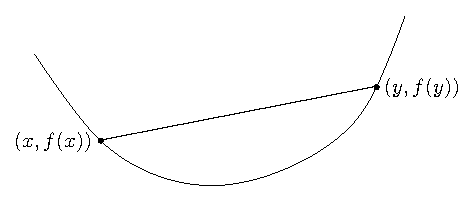
\includegraphics[scale=1,page=1]{fig/note06/03.pdf}
  %\caption{$y = \sin x$,$y = \sin^{-1} x$}
\end{figure}

\end{frame}

\begin{frame}{Example Functions on $\mathbb{R}$}

\begin{itemize}
  \item convex functions
    \begin{itemize}
      \item affine: $\ds ax + b$, $\forall\,a,\;b\in\mathbb{R}$
      \item exponential: $\ds e^{a x}$, $\forall\,a\in\mathbb{R}$
      \item power: $\ds x^\alpha$ on $x > 0$, $\forall\,\alpha\geqslant 1\,\vee\,\alpha\leqslant 0$
      \item power of absolute value: $\ds |x|^\alpha$, $\forall\,\alpha\geqslant 1$
      \item positive part (relu): $\max\{x, 0\}$
    \end{itemize}
  \item concave functions
    \begin{itemize}
      \item affine: $\ds ax + b$, $\forall\,a,\;b\in\mathbb{R}$
      \item power: $\ds x^\alpha$ on $x > 0$, $\forall\,0\leqslant\alpha\leqslant 1$
      \item logarithm: $\ds\log x$ on $x > 0$
      \item entropy: $\ds -x\log x$ on $x > 0$ 
      \item negative part: $\min\{x, 0\}$
    \end{itemize}
\end{itemize}

\end{frame}

\begin{frame}{Example Convex Functions on $\mathbb{R}^n$}

\begin{itemize}
  \item affine: $\ds a^\top\!x + b$
  \item any norm 
    \begin{itemize}
      \item $\ds\|x\|_p = \big(|x_1|^p + |x_2|^p + \cdots + |x_n|^p\big)^{\frac{1}{p}}$, $\forall\,p > 1$
      \item $\ds\|x\|_\infty = \max\,\{|x_1|, |x_2|,\,\ldots\,,|x_n|\}$
    \end{itemize}
  \item sum of squares: $\ds\|x\|_2^2 = x_1^2 + x_2^2 + \cdots + x_n^2$
  \item max function: $\ds\max(x) = \max\,\{x_1, x_2,\,\ldots\,,x_n\}$
  \item softmax / log-sum-exp: $\ds\log\big(e^{x_1} + e^{x_2} + \cdots + e^{x_n}\big)$
\end{itemize}

\end{frame}

\begin{frame}{Example Functions on $\mathbb{R}^{m\times n}$}

\begin{itemize}
  \item Let $\ds X\in\mathbb{R}^{m\times n}$ be the variable
  \item general affine function
    \begin{align*}
      f(X) = \tr(A^\top X) + b = \sum_{i=1}^m\sum_{j=1}^n A_{ij} X_{ij} + b, \quad A\in\mathbb{R}^{m\times n},\;b\in\mathbb{R}
    \end{align*}
  \item spectral norm (maximum singular value) is convex: 
    \begin{align*}
      f(X) = \|X\|_2 = \sigma_{\text{max}}(X) = \sqrt{\lambda_{\text{max}}(X^\top X)}
    \end{align*}
  \item log determinant is concave:
    \begin{align*}
      f(X) = \log\det X, \quad X\in\mathsf{S}^n_{++}
    \end{align*}
\end{itemize}
\end{frame}

\begin{frame}{Extended-Value Extension}
  \begin{itemize}
    \item suppose $f$ is convex on $\mathbb{R}^n$
    \item its extended-value extension $\ds\widetilde{f}: \mathbb{R}^n\to\mathbb{R}\cup\{\infty\}$ is defined as
      \begin{align*}
        \widetilde{f}(x) = \begin{cases}f(x) & x\in\dom f \\ \infty & x\not\in\dom f\end{cases} 
      \end{align*}
    \item this often simplifies notation; e.g. the condition 
      \begin{align*}
        0\leqslant\theta\leqslant 1\ie\widetilde{f}(\theta x + (1 - \theta) y)\leqslant\theta\widetilde{f}(x) + (1 - \theta)\widetilde{f}(y)
      \end{align*}
      (as an inequality in $\mathbb{R}\cup\{\infty\}$), means the same as the two conditions combine
      \begin{itemize}
        \item $\dom f$ is convex
        \item $x,\,y\in\dom f,\;0\leqslant\theta\leqslant 1 \ie f(\theta x + (1 - \theta)y)\leqslant\theta f(x) + (1 - \theta) f(y)$
      \end{itemize}
  \end{itemize}
\end{frame}

\begin{frame}{Restriction of a Convex Function to a Line}

\begin{itemize}
  \item $f:\mathbb{R}^n\to\mathbb{R}$ is convex (concave) $\ifff$ $g:\mathbb{R}\to R$, 
    \begin{align*}
      g(t) = f(x + t\,v), \quad\dom g = \{t\,|\, x+t\,v\in\dom f\}  
    \end{align*}
    is convex (concave) in $t$ for all $x\in\dom f$ and $v\in\mathbb{R}^n$
  \item useful for checking convexity / concavity of multivariate $f$; e.g. to check the concavity of log determinant: Let $X\in\mathsf{S}^n_{++}$, $V\in\mathsf{S}^n$,
    \begin{align*} 
      g(t) &= f(X + t\,V) = \log\det(X + t\,V) \\
           &= \log\det\big(X^{\frac{1}{2}}\big(I + t\,X^{-\frac{1}{2}}VX^{-\frac{1}{2}}\big)X^{\frac{1}{2}}\big) \\
           &= \log\det X + \log\det\big(I + t\,X^{-\frac{1}{2}}VX^{-\frac{1}{2}}\big) \\
           &= \log\det X + \sum_{i=1}^n\log(1 + t\lambda_i) 
         \end{align*}\vspace{-3em}
    where $\lambda_i$ are the eigenvalues of $\ds X^{-\frac{1}{2}}VX^{-\frac{1}{2}}$; $g$ is concave in $t$
\end{itemize}

\end{frame}

\begin{frame}{First-Order Condition}

\begin{itemize}
  \item $f:\mathbb{R}^n\to\mathbb{R}$ is twice differentiable if $\dom f$ is open and the gradient $\nabla f$ exists at each $x\in\dom f$.
  \item {\bf first-order condition} differentiable $f$ with convex domain is convex $\ifff$ $\ds f(y) \geqslant f(x) + \nabla f(x)^\top(y - x),\;\forall\,x,\,y\in\dom f$
  \item first order Taylor approximation of convex $f$ is a {\bf global underestimator} of $f$
\end{itemize}
\begin{figure}[!htbp]
  \centering
  \includegraphics[scale=1,page=2]{fig/note06/03.pdf}
  %\caption{$y = \sin x$,$y = \sin^{-1} x$}
\end{figure}

\end{frame}

\begin{frame}{Second-Order Condition}

\begin{itemize}
  \item $f:\mathbb{R}^n\to\mathbb{R}$ is {\bf differentiable} if $\dom f$ is open and the Hessian matrix $\nabla^2 f\in\mathsf{S}^n$ exists at each $x\in\dom f$: 
    \begin{align*}
      \big\{\nabla^2 f(x)\big\}_{ij} = \frac{\partial^2 f}{\partial x_i\partial x_j}(x)
    \end{align*}
  \item {\bf second-order condition} for twice differentiable $f$ with convex domain is convex: 
    \begin{itemize}
      \item $f$ is convex $\ifff$ $\nabla^2 f\succcurlyeq 0$, $\forall\,x\in\dom f$
      \item $\nabla^2 f\succ 0$, $\forall\,x\in\dom f$ $\ie$ $f$ is strictly convex
    \end{itemize}
\end{itemize}

\end{frame}

\begin{frame}{Examples}

\begin{itemize}
  \item {\bf quadratic function}: $\ds f(x) = \frac{1}{2}\,x^\top P x + q^\top x + r$ with $P\in\mathsf{S}^n$ 
    \begin{align*}
      \nabla f(x) = P x + q,\quad \nabla^2 f(x) = P
    \end{align*}
    convex if $P\succcurlyeq 0$ (concave if $P\preccurlyeq 0$)
  \item {\bf least-squares objective}: $\ds f(x) = \|A\,x - b\|^2$ 
    \begin{align*}
      \nabla f(x) = 2A^\top(A\,x - b),\quad \nabla^2 f(x) = 2 A^\top A 
    \end{align*}
    convex for any $A$
  \item {\bf quadratic-over-linear function}: $\ds f(x, y) = \frac{x^2}{y}$, $y > 0$ 
    \begin{align*}
      \nabla f(x, y) = \begin{pmatrix}\frac{2x}{y} & -\frac{x^2}{y^2}\end{pmatrix},\quad \nabla^2 f(x, y) = \frac{2}{y^3}\begin{pmatrix}y^2 & -xy \\ -xy & x^2 \end{pmatrix}
    \end{align*}
    convex for $y > 0$
\end{itemize}

\end{frame}

\begin{frame}
\begin{figure}[!htbp]
  \centering
  \includegraphics[scale=1.1,page=3]{fig/note06/03.pdf}
  \caption{Graph of quadratic-over-linear function $\ds f(x, y) = \frac{x^2}{y}$, $y > 0$}
\end{figure}

\begin{itemize}
  \item {\bf log-sum-exp function}: $\ds f(x) = \log\Big(\sum_{k = 1}^n e^{x_k}\Big)$ is convex:
    \begin{align*}
      \nabla^2 f(x) = \frac{1}{\symbfup{1}^\top z}\diag(z) - \frac{1}{(\symbfup{1}^\top z)^2}zz^\top, \quad z_k = e^{x_k}
    \end{align*}
  \item to show that $\nabla^2 f(x)\succcurlyeq 0$, one must verify $\ds v^\top\nabla^2 f(x)\,v\geqslant 0\;\forall\,v$:
    \begin{align*}  
      v^\top\nabla^2 f(x)\,v = \frac{\big(\sum_k z_k v_k^2\big)\big(\sum_k z_k\big) - \big(\sum_k v_k z_k\big)^2}{\big(\sum_k z_k\big)^2}\geqslant 0
    \end{align*}
  by Cauchy-Schwarz inequality $\ds \big(\sum_k z_k v_k^2\big)\big(\sum_k z_k\big) \geqslant \big(\sum_k v_k z_k\big)^2$
  \item {\bf geometric-mean function}: $\ds f(x) = \Big(\prod_{k = 1}^n x_k\Big)^{\frac{1}{n}}$ on $x\succ 0$ is concave
\end{itemize}
\end{frame}

\begin{frame}{Epigraph, Sublevel Set}
\begin{itemize}
  \item {\bf $\alpha$-sublevel set} of $f:\mathbb{R}^n\to\mathbb{R}$: $\ds C_\alpha = \{x\in\dom f\,|\, f(x)\leqslant\alpha\}$
  \item sublevel sets of convex functions are convex sets
  \item {\bf epigraph} of $f: \mathbb{R}^n\to\mathbb{R}$: \\ $\ds\epi f = \{(x, t)\in\mathbb{R}^{n+1}\,|\,x\in\dom f,\; f(x)\leqslant t\}$
  \item $f$ is convex $\ifff$ $\ds\epi f$ is a convex set
\end{itemize}
\begin{figure}[!htbp]
  \centering
  \includegraphics[scale=0.8,page=5]{fig/note06/03.pdf}
\end{figure}

\end{frame}

\begin{frame}{Jensen's Inequality}

\begin{itemize}
  \item {\bf basic form}: if $f$ is convex, then for $x$, $y\in\dom f$, $0\leqslant\theta\leqslant 1$
    \begin{align*}
      f(\theta x + (1 - \theta) y) \leqslant \theta f(x) + (1 - \theta) f(y)
    \end{align*}
  \item {\bf extension}: if $f$ is convex and $z$ is a random variable on $\dom f$,
    \begin{align*}
      f\big(\expc{z}\,\big) \leqslant \expc{f(z)}
    \end{align*}
  \item basic form is special case with discrete distribution
    \begin{align*}
      \prb\{z = x\} = \theta,\quad\prb\{z = y\} = 1 - \theta
    \end{align*}
  \item e.g. for $\ds z\sim\mathsf{N}(\mu,\sigma^2)$, let $\ds f(x) = e^x$, then
    \begin{align*}
      f\big(\expc{z}\,\big) = f(\mu) = e^{\mu}\leqslant e^{\mu + \frac{\sigma^2}{2}} = \expc{f(z)}
    \end{align*}
\end{itemize}

\end{frame}

\begin{frame}{Showing Convexity of a Function}

\begin{itemize}
  \item apply definition (often simplified by restricting to a line)
  \item for twice differentiable functions, show $\ds\nabla^2 f(x)\succcurlyeq 0$
  \item show that $f$ is obtained from simple convex functions by operations that preserve convexity
    \begin{itemize}
      \item nonnegative multiple, sum, integral
      \item composition with affine function
      \item pointwise maximum and supremum
      \item partial minimization
      \item composition
      \item perspective
    \end{itemize}
\end{itemize}

\end{frame}

\begin{frame}{Nonnegative Multiple, Sum, Integral}
\begin{itemize}
  \item {\bf nonnegative multiple}: $\alpha f$ is convex if $f$ is convex and $\alpha\geqslant 0$
  \item {\bf sum}: $f_1 + f_2$ is convex if $f_1$, $f_2$ is convex
  \item {\bf infinite sum}: if each of $\ds f_i$ is convex, then $\ds\sum_{i = 1}^\infty f_i$ is convex
  \item {\bf integral}: if $\ds f(x, \alpha)$ is convex in $x$ for each $\alpha\in\mathcal{A}$, then 
    \begin{align*}
      \int_{\alpha\in\mathcal{A}}f(x,\alpha)\,\text{d}\alpha
    \end{align*} 
    is convex
  \item analogous rules for concave functions
\end{itemize}

\end{frame}

\begin{frame}{Composition with Affine Function}

\begin{itemize}
  \item $\ds f(A\,x + b)$ is convex if $f$ is convex
  \item e.g.
    \begin{itemize}
      \item log barrier for linear inequalities
        \begin{align*}
          f(x) &= - \sum_{i = 1}^m \log\big(b_i - a_i^\top x\big) \\
          \dom f &= \{x\,|\,a_i^\top x < b_i,\;i=1,2,\ldots,m\}
        \end{align*}
      \item norm approximation error (any norm)
        \begin{align*}
          f(x) = \|A\,x - b\|
        \end{align*}
    \end{itemize}
\end{itemize}

\end{frame}

\begin{frame}{Pointwise Maximum}

\begin{itemize}
  \item $\ds f(x) = \max\,\{f_1(x),f_2(x),\,\ldots,f_m(x)\}$ is convex if each $f_i$ is convex
  \item e.g.
    \begin{itemize}
      \item piecewise linear function
        \begin{align*}
          f(x) = \max_i\big(a_i^\top x + b_i\big)
        \end{align*}
      \item sum of $r$ largest components of $x\in\mathbb{R}^n$  
        \begin{align*}
          f(x) = x_{[1]} + x_{[2]} + \cdots + x_{[r]}
        \end{align*}
        where $x_{[i]}$ is $i$-th largest component of $x$. Note that
        \begin{align*}
          f(x) = \max\,\{x_{i_1} + x_{i_2} + \cdots + x_{i_r}\,|\,1\leqslant i_1 < i_2 < \cdots < i_r\leqslant n\}
        \end{align*}
    \end{itemize}
\end{itemize}

\end{frame}

\begin{frame}{Pointwise Supremum}

\begin{itemize}
  \item $\ds g(x) = \sup_{y\in\mathcal{A}}f(x, y)$ is convex if $f(x, y)$ is convex in $x$ for each $y\in\mathcal{A}$
  \item e.g.
    \begin{itemize}
      \item distance to farthest point in a set $C$
        \begin{align*}
          f(x) = \sup_{y\in C}\,\|x - y\|
        \end{align*}
      \item maximum eigenvalue of symmetric matrix 
        \begin{align*}
          \lambda_{\text{max}}(X) = \sup_{\|y\|_2 = 1} y^\top X\,y, \quad X\in\mathsf{S}^n 
        \end{align*}
      \item support function of a set $C$
        \begin{align*}
          S_C(x) = \sup_{y\in C}\,y^\top x
        \end{align*}
    \end{itemize}
\end{itemize}

\end{frame}

\begin{frame}{Partial Minimization}

\begin{itemize}
  \item the function $\ds g(x) = \inf_{y\in C} f(x, y)$ is called the {\bf partial minimization} of $f$ w.r.t. $y$
  \item if $f(x, y)$ is convex in $(x, y)$ and $C$ is a convex set, then partial minimization $g$ is convex
  \item e.g.
    \begin{itemize}
      \item let $f(x, y) = x^\top A\,x + 2 x^\top B\,y + y^\top C\,y\;$ with $\ds\;\begin{pmatrix}A & B \\ B^\top & C\end{pmatrix}\succcurlyeq 0$, $C\succ 0$; minimizing over $y$ gives 
        \begin{align*}
          g(x) = \inf_{y\in C}\,f(x, y) = x^\top\big(A - BC^{-1}B^\top\big)\,x
        \end{align*}
        $g$ is convex, hence Schur complement $A - BC^{-1}B^\top\succcurlyeq 0$
      \item distance to a convex set $S$
        \begin{align*}
          \dist(x, S) = \inf_{y\in S}\,\|x - y\|
        \end{align*}
    \end{itemize}
\end{itemize}

\end{frame}

\begin{frame}{Composition with Scalar Functions}

\begin{itemize}
  \item composition of $g:\mathbb{R}^n\to\mathbb{R}$ and $h:\mathbb{R}^n\to\mathbb{R}$ is $\ds f(x) = h(g(x))$ ($\ds f = h\circ g$)
  \item composition $f$ is convex if
    \begin{itemize}
      \item $g$ convex, $h$ convex, $\ds\widetilde{h}$ nondecreasing; or
      \item $g$ concave, $h$ convex, $\ds\widetilde{h}$ nonincreasing
    \end{itemize}
  \item proof for $n = 1$, differentiable $g$, $h$
    \begin{align*}
      f''(x) = h''(g(x))\,g'(x)^2 + h'(g(x))\,g''(x)
    \end{align*}
  \item e.g.
    \begin{itemize}
      \item $f(x) = e^{g(x)}$ is convex if $g$ is convex
      \item $\ds f(x) = \frac{1}{g(x)}$ is convex if $g$ is concave and positive
    \end{itemize}
\end{itemize}

\end{frame}

\begin{frame}{Composition: General}

\begin{itemize}
  \item composition of $g:\mathbb{R}^n\to\mathbb{R}^k$ and $h:\mathbb{R}^n\to\mathbb{R}$ is $\ds f(x) = h(g_1(x), g_2(x),\ldots, g_k(x))$
  \item composition $f$ is convex if $h$ is convex and for each $i$, one of the following holds:
    \begin{itemize}
      \item $g_i$ convex, $\ds\widetilde{h}$ nondecreasing in its $i$-th argument
      \item $g_i$ concave, $\ds\widetilde{h}$ nonincreasing in its $i$-th argument
      \item $g_i$ affine
    \end{itemize}
  \item e.g.
    \begin{itemize}
      \item $\ds\log\Big(\sum_{i = 1}^m e^{g_i(x)}\Big)$ is convex if each $g_i$ is convex
      \item $\ds\frac{p(x)^2}{q(x)}$ is convex if $p$ is nonnegative and convex and $q$ is positive and concave
    \end{itemize}
\end{itemize}

\end{frame}

\begin{frame}{Perspective}

\begin{itemize}
  \item perspective of $f:\mathbb{R}^n\to\mathbb{R}$ is the function $\ds g(x, t):\mathbb{R}^n\times\mathbb{R}\to\mathbb{R}$ defined as 
    \begin{align*}
      g(x, t) = t\,f\Big(\frac{x}{t}\Big), \quad\dom g = \Big\{(x, t)\;\Big|\;\frac{x}{t}\in\dom f,\;t > 0\Big\}
    \end{align*}
  \item $g$ is convex if $f$ is convex
  \item e.g.
    \begin{itemize}
      \item $\ds f(x) = x^\top x$ is convex, so $\ds g(x, t) = \frac{x^\top x}{t}$ is convex if $t > 0$
      \item $\ds f(x) = -\log x$ is convex, so the {\bf relative entropy} 
        \begin{align*}
          g(x, t) = t\,\log t - t\,\log x
        \end{align*} 
        is convex on $x > 0$, $t > 0$ 
    \end{itemize}
\end{itemize}

\end{frame}

\begin{frame}{Convexity Verification: An Example}

\begin{itemize}
  \item test the convexity of $\ds f(x, y) = \frac{(x - y)^2}{1 - \max(x, y)}, \; x < 1,\;y < 1$
  \item $x$, $y$, and $1$ are affine
  \item $\max(x, y)$ is convex; $x - y$ is affine
  \item $1 - \max(x, y)$ is concave
  \item $\ds\frac{u^2}{v}$ is convex, monontone decreasing in $v$ for $v > 0$
  \item $f$ is composition of $\ds\frac{u^2}{v}$ with $u = x - y$, $v = 1 - \max(x, y)$, hence convex
\end{itemize}

\end{frame}

\begin{frame}{Convexity Verification: A Caveat}

\begin{itemize}
  \item test the convexity of $\ds f(x) = \sqrt{1 + x^2}$
  \item $\sqrt{\cdot}$ is concave 
  \item $1$, $x^2$ are convex 
  \item $\sqrt{1 + x^2}$ is $\,\ldots\,$ indefinite ?
  \item but, note that $\ds\|\cdot\|_2$ is convex
  \item $\ds\sqrt{1 + x^2}$ can be represented as the 2-norm of vector $(1, x)$ --- $\ds\|(1, x)\|_2$, hence is convex
  \item The general composition rules are only sufficient, not necessary
\end{itemize}

\end{frame}

%\subbegin{frame}{Outline}
%\begin{frame}
%  \tableofcontents
%\end{frame}

%\begin{frame}[allowframebreaks]
%  \frametitle{References}
%  \nocite{*}
%  \bibliographystyle{apalike}
%  \bibliography{note06}
%\end{frame}

\end{document}
